% Author : Juan Garcia Garland
% LIcense: GPLv3 

\documentclass{beamer}

\usetheme{Rochester}
\usefonttheme[onlymath]{serif}
\usepackage{bussproofs}

\usepackage{qcircuit}
\usepackage{braket}

\begin{document}
\title{Algoritmo de Shor} 
\author{Juan Pablo Garc\'ia Garland} 
\date{Mayo, 2018} 

\frame{\titlepage} 

\frame{\frametitle{\'Indice}
  \tableofcontents
}


%\section{Intro}
%%intro, simon algorithm


\frame{
  Problema: Sea $f:\mathbb{B}^n\rightarrow\ \mathbb{B}^n$,
  y $s \in \mathbb{B}^n$, donde $f(x) = f(x \oplus s)$
  \pause
  Soluci\'on cl\'asica:
  \begin{itemize}
  \item $f$ es una funci\'on gen\'erica, no podemos
    hacer m\'as que evaluarle.
  \item Potencialmente el recorrido de $f$ tiene cardinal $2^{n-1}$.
  \item Para encontrar dos im\'agenes distintas
    necesitamos potencialmente $ o(2^{\frac{n}{2}})$ evaluaciones.
  \end{itemize}
}

\frame{
  
  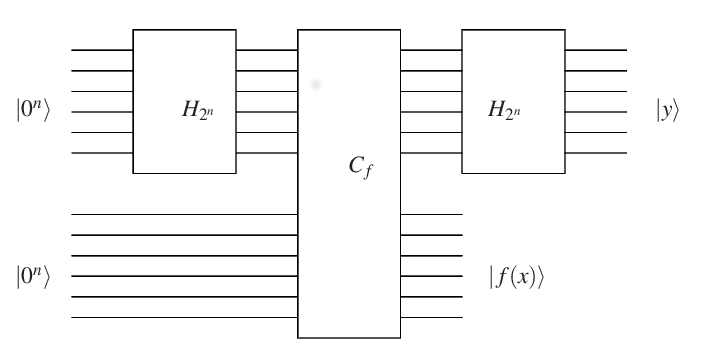
\includegraphics[scale=0.4]{./graphics/simon}
}

\frame{


  $\left(\begin{array}{rrrrrrrr}
1 & 1 & 1 & 1 & 1 & 1 & 1 & 1 \\
1 & \left(\frac{1}{2} i + \frac{1}{2}\right) \, \sqrt{2} & i
& \left(\frac{1}{2} i - \frac{1}{2}\right) \, \sqrt{2} & -1
& -\left(\frac{1}{2} i + \frac{1}{2}\right) \, \sqrt{2} & -i
& -\left(\frac{1}{2} i - \frac{1}{2}\right) \, \sqrt{2} \\
1 & i & -1 & -i & 1 & i & -1 & -i \\
1 & \left(\frac{1}{2} i - \frac{1}{2}\right) \, \sqrt{2} & -i
& \left(\frac{1}{2} i + \frac{1}{2}\right) \, \sqrt{2} & -1
& -\left(\frac{1}{2} i - \frac{1}{2}\right) \, \sqrt{2} & i
& -\left(\frac{1}{2} i + \frac{1}{2}\right) \, \sqrt{2} \\
1 & -1 & 1 & -1 & 1 & -1 & 1 & -1 \\
1 & -\left(\frac{1}{2} i + \frac{1}{2}\right) \, \sqrt{2} & i
& -\left(\frac{1}{2} i - \frac{1}{2}\right) \, \sqrt{2} & -1
& \left(\frac{1}{2} i + \frac{1}{2}\right) \, \sqrt{2} & -i
& \left(\frac{1}{2} i - \frac{1}{2}\right) \, \sqrt{2} \\
1 & -i & -1 & i & 1 & -i & -1 & i \\
1 & -\left(\frac{1}{2} i - \frac{1}{2}\right) \, \sqrt{2} & -i
& -\left(\frac{1}{2} i + \frac{1}{2}\right) \, \sqrt{2} & -1
& \left(\frac{1}{2} i - \frac{1}{2}\right) \, \sqrt{2} & i &
\left(\frac{1}{2} i + \frac{1}{2}\right) \, \sqrt{2}
\end{array}\right)$


}



\section{Parte cl\'asica: Reducci\'on de Factorizaci\'on a order finding}
\frame{Factorizaci\'on}

\frame{
\frametitle{Factorizacion}
\framesubtitle{Reducci\'on a order finding}

  Sea $n \in \mathbb{N} $, con $N = pq$, $p$ y $q$ primos "grandes".
  \pause
  
  Consideramos la ecuaci\'on:
  $$x^2 \equiv 1\mod N$$
  \pause
  
  Es equivalente a
  $$N \vert \left( x+1 \right) \left( x-1 \right)$$
  \pause

  Si $x \not\equiv \pm 1$ entonces $p \vert ( x+1 ) $ y $q \vert ( x-1 )$
  (s.p.d.g.).
  \pause
  
  De hecho $p = gcd(x+1,N)$, $q=gcd(x-1, N)$
}  


\section{Order finding a Period Finding}
\frame{\frametitle{Factorizaci\'on}
\framesubtitle{Order Finding}
Sea $x\in\mathbb{N}$, con $m \perp N$. \pause

Si existe una forma eficiente
de calcular $O(m)$, y es par, entonces tomamos $x = m^{\frac{O(m)}{2}}$.
\pause

Tomando un $m$ arbitrario,
?`Cu\'al es la probabilidad de que $O(m)$ sea par y $x$ no trivial?\pause

\huge{ALTA}
}

\frame{\frametitle{Order Finding}
\framesubtitle{Period finding}
Encontrar el \'orden de $m$ es an\'alogo a encontrar el per\'iodo de
$f(n) = m^n$
}







\section{Transformada de Fourier}

\frame{\frametitle{Transformada de Fourier (Discreta).}

  Definici\'on: La $DFT$ es una funci\'on de tipo
  $\mathbb{C}^N\rightarrow\mathbb{C}^N$.
  
  Si $X_0, \cdots X_{N-1}$ es una secuencia de $N$ n\'umeros
  complejos y $Y_0, \cdots Y_{N-1}$ la transformada, se cumple que:
  $$
  Y_i = \sum_{j=0}^{N-1}{X_j \omega^{ij}}
  $$
  Donde $\omega = e^{i \frac{2\pi}{N}}$ es una ra\'iz \emph{primitiva}
  $N-$\'esima de la unidad.
}


\frame{\frametitle{Transformada de Fourier (Discreta).}
  Si consideramos $X_1 \cdots X_{N-1}$ como vector,
  hacer la DFT es multiplicar por la matriz:

  {
    %blob
    $\displaystyle DFT_n={\begin{bmatrix}1&1&1&1&\cdots &1\\1&\omega &\omega ^{2}&\omega ^{3}&\cdots &\omega ^{N-1}\\1&\omega ^{2}&\omega ^{4}&\omega ^{6}&\cdots &\omega ^{2(N-1)}\\1&\omega ^{3}&\omega ^{6}&\omega ^{9}&\cdots &\omega ^{3(N-1)}\\\vdots &\vdots &\vdots &\vdots &\ddots &\vdots \\1&\omega ^{N-1}&\omega ^{2(N-1)}&\omega ^{3(N-1)}&\cdots &\omega ^{(N-1)(N-1)}\end{bmatrix}}$
}}

\frame{\frametitle{Transformada de Fourier (Cu\'antica).}
  Consideramos la transformaci\'on unitaria:
  $$QFT_N={\frac{1}{\sqrt{N}}\begin{bmatrix}1&1&1&1&\cdots &1\\1&\omega &\omega ^{2}&\omega ^{3}&\cdots &\omega ^{N-1}\\1&\omega ^{2}&\omega ^{4}&\omega ^{6}&\cdots &\omega ^{2(N-1)}\\1&\omega ^{3}&\omega ^{6}&\omega ^{9}&\cdots &\omega ^{3(N-1)}\\\vdots &\vdots &\vdots &\vdots &\ddots &\vdots \\1&\omega ^{N-1}&\omega ^{2(N-1)}&\omega ^{3(N-1)}&\cdots &\omega ^{(N-1)(N-1)}\end{bmatrix}}$$

  A este circuito/programa lo llamamos $QFT_N$.
}

\frame{
  Notar que $QFT_N$ act\'ua sobre un estado cu\'antico
  en un sistema de $N$ niveles (vector normalizado),
  y $DFT_N$ sobre un vector arbitrario.\pause
  
  $QFT$ es un operador unitario, $DFT$ no necesariamente,
  por lo dem\'as van a cumplir propiedades similares.
  
}


\frame{\frametitle{Transformada de Fourier Cu\'antica.}
       \framesubtitle{Propiedades de la FT}
  Es unitaria.
}  
\frame{\frametitle{Transformada de Fourier Cu\'antica.}
       \framesubtitle{Propiedades de la FT}
  Si hacemos un shift en la entrada,
  los m\'odulos de la salida no cambian.
}

\frame{\frametitle{Transformada de Fourier Cu\'antica.}
    \framesubtitle{Propiedades de la FT}
  Para una $QFT_{nk}$
  Si la entrada es una funci\'on de $k$ per\'iodos,
  la salida tiene valores no nulos en los m\'ultiplos de $n$.
}

\frame{\frametitle{Transformada de Fourier (Discreta).}
    \framesubtitle{Propiedades de la FT}
  Un caso m\'as restrictivo.
}



\section{Period finding}
\frame{TODO}

\section{Algoritmo de Shor}
\frame{}

\end{document}


